\documentclass[border=10pt]{standalone}
\usepackage{tikz}
\usetikzlibrary{arrows.meta, positioning}

\begin{document}

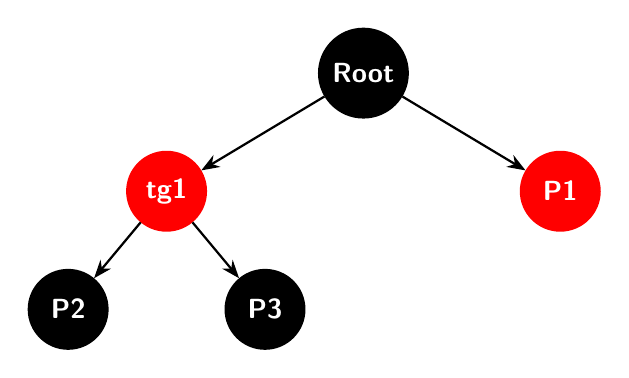
\begin{tikzpicture}[
    ->, >=Stealth, thick,
    level distance=1.5cm,
    level 1/.style={sibling distance=5cm},
    level 2/.style={sibling distance=2.5cm},
    bnode/.style={circle, draw=black, fill=black, text=white, minimum size=1cm, font=\bfseries\sffamily},
    rnode/.style={circle, draw=red, fill=red, text=white, minimum size=1cm, font=\bfseries\sffamily},
    nilnode/.style={rectangle, draw=black, fill=black, text=white, minimum size=0.6cm, font=\sffamily\scriptsize}
]


\node [bnode] {Root}
    child { node [rnode] {tg1}
        child { node [bnode] {P2} }
        child { node [bnode] {P3} }
    }
    child { node [rnode] {P1} };

\end{tikzpicture}

\end{document}